To conclude, the fixed goal mode RL problems have been more or less solved
by all evaluated policies.
With a one dimensional action space, both policies learn precise decision making 
in an appropriate amount of steps. Especially the policy derived from the PPO algorithms
quickly converges to a local optimum and shows steady performance.
In comparison, the SACs performance is much more unsteady due to it being off-policy.
Both policies show convincing results across the entire metric.
However, due to the one dimensional action space, the drone is limited to 
translational movements along the $z$ axis.\\
When increasing the dimension of the action space to 4 dimensions, the 
complexity of the task increases immensely and more training steps
are needed in order to achieve adequate performance.
While the SAC algorithms performance seems to converge, the PPO performance
decreases again, which indicates that the policy derived from PPO has problems 
at generalizing this task.
Overall, the actions of the four dimensional policies seem to mimic
the one dimensional action making. However, even small differences leads
to error that have to be corrected later on. 
Especially near the point the action making gets noisy.
Although the PPO policy outperforms the SAC policy on the raw metric,
it does not show preferable flight control.
It shows a constant yaw velocity and causes crashing when increasing the episode length.
This also indicates, that PPO does not generalize the task well.
Also, it is not robust to a change in the control frequency.
In contrast, the policies derived from the SAC algorithm seems to be robust
to the control frequency. In addition, the SAC performance does not seem to be 
dependent on the control frequency during training.\\
On random goal modes, the performance drops significantly.
Especially LCL has some inherit problems, caused by the linearization. As a consequence,
even a normal learning without any curriculum shows better results, although
even these are of poor quality.
However, it should be said that neither method was really fine-tuned due to limitation
of time during this work. Still, on some goals, 
the policies show a good performance like seen in the Appendix B, but there is no sign of 
generalization in either of those.\\
When evaluating the policies on environments with harsh conditions, it can be observed that 
learning them without wind is not good enough for stable flight, because the state space was not explored enough, and the policies do not optimize safety.\\
In the following section some ideas will be introduced, that might help to
overcome the current difficulties.

\newpage

\section{Of Migrating to a real Drone}
It was already presented \cref{sec: autoquad} how the intelligent agents presented in 
this work may be used in a real intelligent flight control.
In order to migrate to a real drone, first an accurate drone model has to be created
and used in combination with the presented scripts, environments, etc. in order to 
create an intelligent agent.
Therefore, test can be used in order to approximate the important parameters 
like thrust to weight ratio or maximum rpm.
Then, the agent has to be embedded into the flight control loop,
accurately calculating the normalized inputs according to the designed observation space.
Also, the actions have to be denormalized to the rpm range of the drone.
It must be noted that the chosen hardware must have the ability to set rpm signals 
to the motors and control them accordingly. Also, it is possible to perform an 
empirical study on the relation between RPM signals and the most commonly used
PWM signals.
Then the denormalized actions are applied with the use of ESC and motors.
Also, it is important to use sensors in order to implement a position estimation.
An accurate position estimation is important since optimal observations are assumed
in the simulation.

\section{Of Performance Improvements against turbulent Conditions}
It was already presented that in order to counteract wind fields, the agents have to be learned
on environments with an active wind field in order to learn save flight.
Furthermore, the question arises whether the current wind should be added to the observation space.
In Theory, this should simplify the task of save flight control, however it is hard 
to really approximate the wind later on. In order to calculate the influence 
of the wind in the last step the drone would need to calculate an expected acceleration, velocity and position 
and compare it with possible sensor input. This is computational complex and
with weak wind the sensor noise might influence the state space immensely.
Therefore, I propose to explore the use of CNN, which could use the circles inside the network in order 
to store memory and use it in order to approximate the wind.
Furthermore, a safer flight can be achieved by using curricula for the wind or even use 
Self-Pased Curriculum Learning.
It was also discussed, that a major problem may be that the agents do not explore the 
observation space enough.
It may be overall beneficial to convert the observation space to a local differential reference frame.
For example, approaching the goal $g_0 = (0, 0, 0.5)$ from $p_0 = (0, 0, 0.25)$ 
is the same problem as approaching $g_1 = (0,1, 0.5)$ from $p_1 = (0, 1, 0.5)$.
Also, this proposes the ability to just learn approaching goals inside a sphere around the drone 
and approaching a projection into the sphere if it is outside. By flying towards 
this projection point, the reference sphere would move and over time the goal moves inside the sphere.
As a consequence, training may be shortened and the observation space decreases significantly, which 
may cause a better exploration of the complete observation space.

\begin{figure}
    \centering
    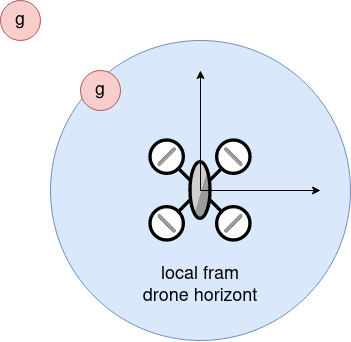
\includegraphics[width=0.55\linewidth]{figures/localframe.png}
    \caption{2D Scratch of local reference horizon with goal and projection (red)}
\end{figure}

\section{Of Improvements in Self-Pased Curriculum Learning}
It was already mentioned that the use of curricula in RL can improve the learning process and 
help to avoid local optima. In this work a linear automation approach was proposed, implemented 
and tested that subdivides the task to reach a random point inside a half ball with a radius $r$
by learning in defined steps with different radii. However, 
this does not seem to be an efficient way.
\cite{klink2021probabilistic} interprets self-paced learning with the KL divergence w.r.t. a
target distribution and shows promising results that help to avoid poor local optima.\\
On the prior described problems, it can be used with different context.
Similar to the LCL the radius distribution would be changed, but based on the current performance
in a way that aims at guaranteeing to keep the performance within a threshold.
Besides, it could be used in order to schedule the wind force of the wind field to 
produce a policy capable of wind-robust flight control.\\
\newline
In total, there are a lot of promising ideas to further improve the presented results
and help to succeed at efficient, universal, safe flight control for flying drones.


%\section{Of hierarchical RL for Sub-Problem-Solving}
%The results of this work clearly shows that with a one directional action space,
%the task can be achieved in very short time with nearly optimal results.
%It should be investigated whether using one dimensional action spaces 
%for $x$ and $y$ axis control can be implemented.
%It should be expected, that the task is more complex than on the $z$ axis
%due to the need of rotation in order to change the $x$ or $y$ position.
%However, if this shows promising results,
%it should be possible to implement a hierarchical RL problem similar to classic
%PID control. In \cref{sec:pid} it was already mentioned that 
%most modern UAVs posses a controller for each axis.
%If this simple controllers can be implemented via RL with promising
%results, then a top level controller can also be learned via RL.
%This top-level controller controls which of the single axis controller should
%be used in order to reach the goal with his action a' (\cref{fig:hiera}).\\
%If the X-Agent is chosen a roll movement is 

%\begin{figure}
%        \begin{subfigure}{0.5 \linewidth} \label{fig:hiera}
%            \includegraphics[width=\linewidth]{figures/hierarchy.png}
%            \subcaption{}
%        \end{subfigure}
%        \hfil
%        \begin{subfigure}{0.5 \linewidth}
%            \includegraphics[width=\linewidth]{figures/hierarchypath.png}
%            \subcaption{}
%        \end{subfigure}
%        \caption{The hierarchical RL concept for UAV flight control (a) and a small 
%        2D visualization of the approximated path (b)}
%\end{figure}
